\section{Attack Taxonomy}\label{attack}

In this section, we describe the considered threat models as well as the methodology and adversary assumptions.
%In this work, we provide a comprehensive privacy analysis of graph embedding algorithms by proposing node membership inference attacks, graph reconstruction attacks and attribute inference attack.


\subsection{Membership Inference Attacks}

Membership Inference attacks allow personal information leakage in GNNs.
Specifically, the goal of the adversary is to identify whether a user node $v$ is part of the graph $G_{train}$ used for training the target model.
This is a binary classification problem where the adversary learns the threshold to predict the membership of a user node.
Depending on the adversary's knowledge about $f()$, we consider two settings: blackbox (with and without auxiliary knowledge) and whitebox. %, based on the adversary's knowledge about $f()$.
As shown Figure~\ref{mia}, to distinguish between members and non-members of training graph $G_{train}$, the blackbox attacks exploit the statistical difference in output predictions while the whitebox attack exploits the intermediate low dimensional embedding.


\begin{figure}[!htb]
\centering
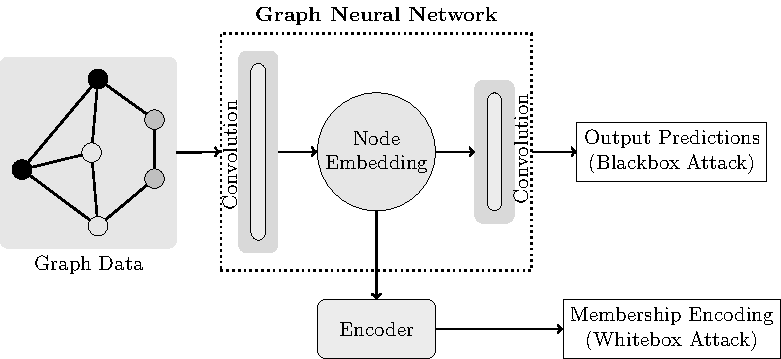
\includegraphics[width=0.85\linewidth]{./figures/Attacks/MIA.pdf}
\caption{Blackbox and Whitebox Inference attacks to distinguish between members and non-members of $G_{train}$.}
\label{mia}
\end{figure}


\subsubsection{Blackbox: Inference using Output Predictions}

%\noindent\textbf{Threat Model.} 
In this setting, we consider the target model as trained GNN for node classification task.
The adversary aims to infer whether a user's node in the graph was used in training the target model $f()$.
In a blackbox setting, adversary has only access to the model outputs $f(x;W)$ for a given input $x$.
The parameters of the trained model $W$ as well as the intermediate computation are inaccessible to the adversary.
This is a practical setting, typically seen in the case of Machine Learning as a Service, where a trained model is deployed in the cloud and the adversary queries the model through an API and receives corresponding predictions.


\begin{figure}[!htb]
    \centering
    \begin{minipage}[b]{1\linewidth}
    \centering
    \subfigure[Citeseer]{
    \label{fig:nonmem_soft_label}
    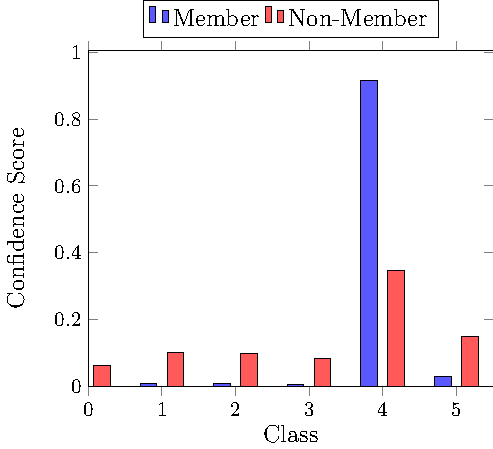
\includegraphics[width=0.5\linewidth]{figures/BBMIA/citeseer_hist.pdf}
    \raisebox{2mm}{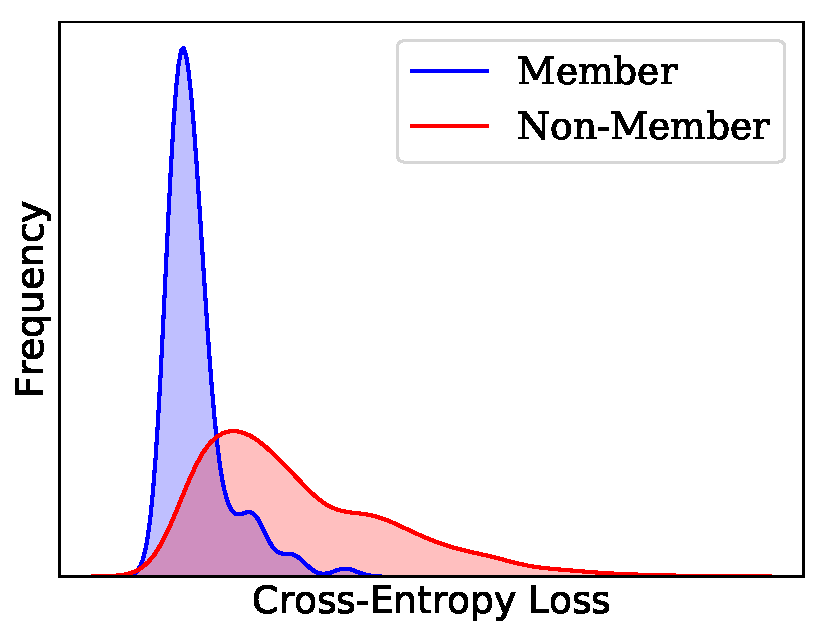
\includegraphics[width=0.5\linewidth]{figures/BBMIA/citeseer.pdf}}
    }

    \subfigure[Cora]{
   	\label{fig:mem_soft_label}
    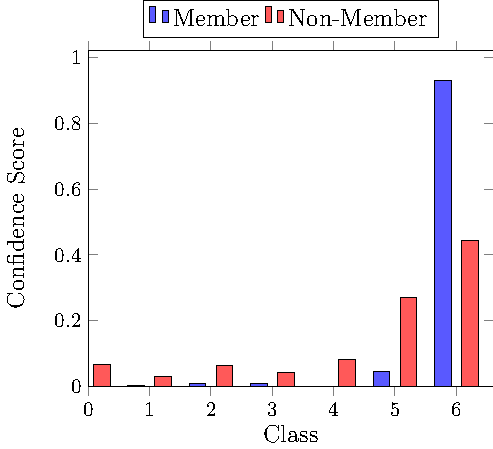
\includegraphics[width=0.5\linewidth]{figures/BBMIA/cora_hist.pdf}
    \raisebox{2mm}{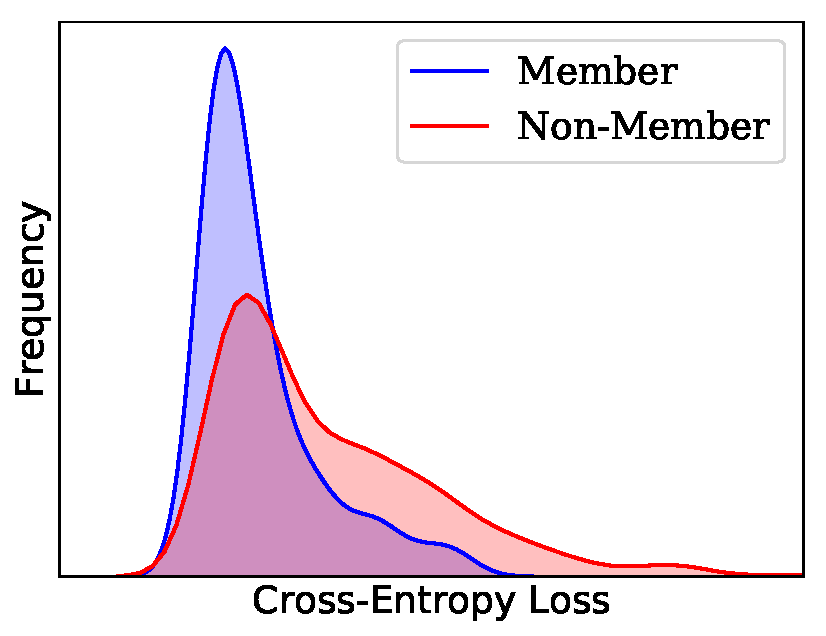
\includegraphics[width=0.5\linewidth]{figures/BBMIA/cora.pdf}}
    }

    \subfigure[Pubmed]{
    \label{fig:mem_soft_label}
    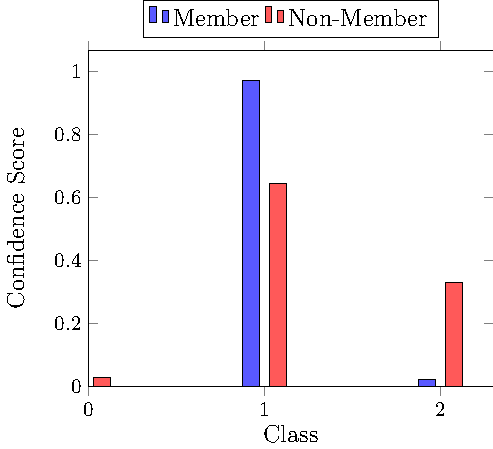
\includegraphics[width=0.5\linewidth]{figures/BBMIA/pubmed_hist.pdf}
    \raisebox{2mm}{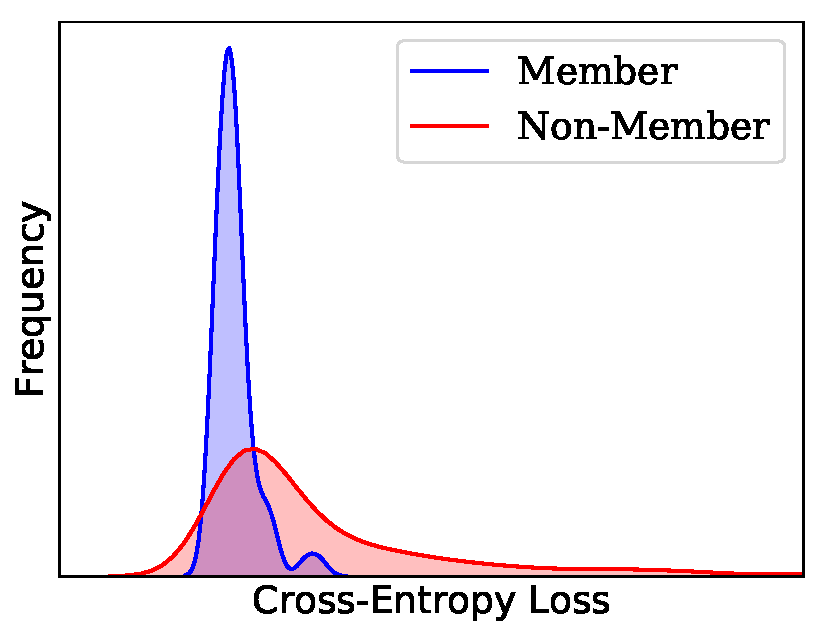
\includegraphics[width=0.5\linewidth]{figures/BBMIA/pubmed.pdf}}
    }
    \end{minipage}
    \caption{Model predictions are more confident for nodes in $G_{train}$ compared to test graph (left). The extent of overfitting can be detected by a non-overlapping region between the output prediction distributions across all data points (right).}
    \label{fig:NIAcause}
\end{figure}

%\noindent\textbf{Attack Motivation.} 
Blackbox adversary exploits the statistical difference between the confidence in prediction on training and testing data~\cite{membershipinf}. % add a reference
Figure~\ref{fig:NIAcause} (left) illustrates this difference where the prediction confidence for one class is much higher for training data points.
Predicting with higher confidence on seen $G_{train}$ nodes compared to unseen test nodes is referred as overfitting.
This difference in the output prediction confidence directly results from a distinguishable output distribution between train and test data indicated by non-overlapping region between distributions (Figure~\ref{fig:NIAcause}, right).


%\noindent\textbf{Attack Methodology.} 
Based on the adversary's auxiliary knowledge about $G_{train}$ distribution, we categorize the attacks into: (a) shadow model attack with auxiliary knowledge of $G_{train}$'s distribution, and (b) confidence score attack with no prior knowledge.\\

\noindent\textbf{Adversary with Auxiliary Knowledge (Shadow Attack):} The adversary is assumed to have an auxiliary graph dataset $G_{aux}$ sampled from the same underlying data distribution as $G_{train}$.
This is a practical assumption where social networks have publicly available API enabling the adversary to obtain subgraphs of the original social network graph.
Further, in this particular work, we assume that the adversary has knowledge about the target GNN architecture which is consistent with prior attack settings~\cite{membershipinf,attributeinf,attributeinf2,logan} but the attack is transferable across different models~\cite{ndss19salem}. 
To conduct its attack, the adversary uses her prior knowledge to map the target model's predictions to membership values and hence the attack is supervised.
For a target model $f()$, the adversary trains a substitute model $f_{local}$ on auxiliary graph data ($G_{aux}$) drawn from the same distribution as $G_{train}$.
The datasets are assumed to be non-overlapping, i.e, $G_{train} \cap G_{aux} = \phi$, which makes the attack more practical.
The goal is to train $f_{local}$ to mimic the behaviour of $f()$, i.e, the output predictions should be similar to each other $f_{local}(v;W') \sim f(v;W)$ for the same input user node $v$ but different parameters $W'$ and $W$ due to training on the different data.
Given the substitute model, the adversary creates a synthetic dataset with binary classes for distinguishing members and non-members (encoded as class 1 and class 0) of $f_{local}$'s training data $G_{aux}$ while using the output predictions as the input features.
That is, the synthetic dataset has the input as $f_{local}$'s predictions for an user node $v$ classified as "Member" if $v \in G_{aux}$ and "Non-Member" otherwise.
Hence, $f_{local}$ is used as a proxy for $f()$ to learn the mapping between the $f()$'s output predictions and the membership information.
The adversary trains a binary attack classifier $f_{attack}$ on the synthetic dataset used to predict whether a new user node was member of $G_{train}$.\\


\begin{figure*}[!htb]
\centering
\resizebox{0.8\textwidth}{!}{
    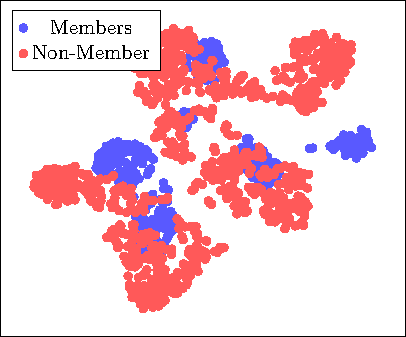
\includegraphics[width=.3\textwidth]{figures/EmbeddingMIA/citeseer.pdf}\hfill
    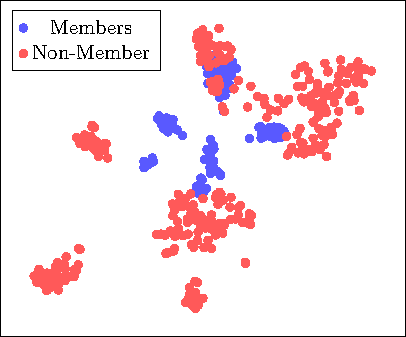
\includegraphics[width=.3\textwidth]{figures/EmbeddingMIA/cora.pdf}\hfill
    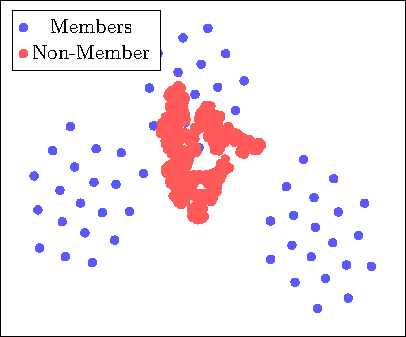
\includegraphics[width=.3\textwidth]{figures/EmbeddingMIA/pubmed.pdf}
  }
\caption{Whitebox membership inference attacks exploit the distinguishable intermediate embedding of train and test graph nodes for Citeseer (left), Cora (middle) and Pubmed dataset (right).}
\label{embedding}
\end{figure*}



\noindent\textbf{Adversary without Auxiliary Knowledge (Confidence Attack):} In this particular case, we alleviate the data distribution assumption of shadow model making the attack applicable to a wide range of practical scenarios.
Since, the adversary does not have prior knowledge to map the output predictions of target model to classify the membership, the attack is performed in an unsupervised setting. %  and does not use shadow or attack model.
To conduct its attack, the adversary leverages the fact that graph nodes with higher output confidence prediction are likely to be members of $G_{train}$.
Here, the adversary finds the output prediction with highest confidence and compares whether this is above a certain threshold to decide whether the corresponding graph node was in the model's training graph $G_{train}$ or not.
A large output confidence indicates membership of the data point in the training data.
The adversary sweeps across different values to select the threshold value which best suits the application.\\





\subsubsection{Whitebox: Inference using Graph Embedding}

%\noindent\textbf{Threat Model.} 
The adversary in a whitebox setting has access to the model output predictions $f(x; W)$ for an input $x$ as well as the model parameters $W$.
This allows the adversary to compute the intermediate computations after each layer which in our case corresponds to the embedding for each node as an output of graph convolutional layer.
This is a strong adversary assumption but practical in the case of federated learning where the intermediate computations and parameters can be observed~\cite{whitebox,collabinf}.

%\noindent\textbf{Attack Motivation.} 
As explained Section~\ref{background}, GNNs compute the low dimensional embedding for the input graph data.
The parameters of GNNs are updated in each iteration of training and are tuned specifically for high performance on the train data resulting in a distinguishable footprint between embedding of train and test data points.
Figure~\ref{embedding} illustrates this rationale by plotting embedding of train and test graph nodes for the three datasets after a dimension reduction using 2D-TSNE algorithm~\cite{tsne}.


%\noindent\textbf{Attack Methodology.} 
The attack is unsupervised as the adversary has no prior knowledge to map the intermediate embeddings to a membership value. % (available as auxiliary knowledge in shadow model).
The adversary trains an encoder-decoder network in unsupervised fashion to map the intermediate embedding to a single membership value.
For an input graph node's embedding $\Psi (v)$, encoder $f_{enc}()$ generates a scalar membership value which is passed to decoder $f_{dec}(f_{enc}(\Psi (v)))$ to obtain $\Psi(v)$ by minimizing reconstruction loss: $||\Psi (v) - f_{dec}(f_{enc}(\Psi (v)))||_2^2$.
Given the membership values for different training and testing data points, K-Means clustering is used to cluster nodes into two classes (members and non-members).
For any new user node, the adversary clusters as members or non-members of the training data.
%This novel whitebox attack exploits the difference in embedding representation between members and non-members of training graph data which is not possible for Deep Neural Networks trained on euclidean data where the intermediate activations are abstract (generalize well) and cannot be used to distinguish members and non-members~\cite{whitebox}.









\subsection{Graph Reconstruction Attack}

%\noindent\textbf{Threat Model.} 
Given a sensitive target graph data ($G_{target}$) and the corresponding set of publicly released embeddings, $\Psi (v)$ $\forall v \in G_{target}$, the goal of the adversary in this attack is to reconstruct $G_{target}$ and the corresponding connections between the different nodes $A_{target}$.
Specifically, the goal of the adversary is to reconstruct the adjacency matrix $A_{target}$ of the graph which is binary with $A_{ij}=1$ if there exists an edge between the node $i$ and $j$ and zero otherwise.
While node membership inference is a subtle privacy violation of user's data, this is a stronger attack where the entire sensitive graph data is reconstructed by the adversary.

%\noindent\textbf{Attack Motivation.} 
Graph embeddings are specially computed to ensure that the underlying graph properties do not change.
In other words, the embeddings capture the rich semantic, invariant and structural information about the graph, for instance, by preserving proximity to the neighbouring nodes.
Hence, there exists a strong correlation between the released graph embeddings and the actual graph which can be exploited to reconstruct the graph data.

\begin{figure}[!htb]
    \centering
    \begin{minipage}[b]{1\linewidth}
    \centering

    \subfigure[Adversary trains attack model on auxiliary subgraph]{
   	\label{fig:mem_soft_label}
    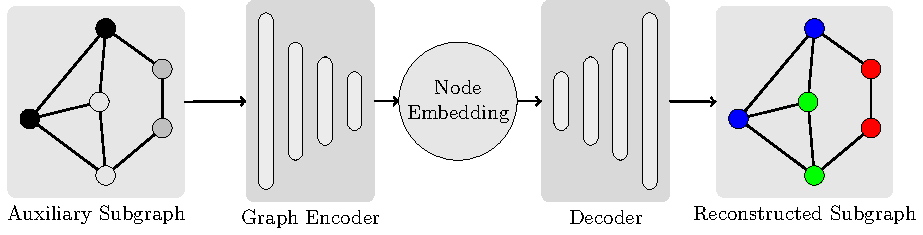
\includegraphics[width=\linewidth]{./figures/Attacks/reconstruction.pdf}
    }

    \subfigure[Attack model reconstructs target graph]{
    \label{fig:mem_soft_label}
    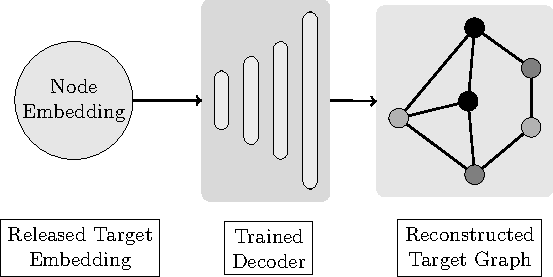
\includegraphics[width=0.6\linewidth]{./figures/Attacks/reconstruction2.pdf}
    }
    \end{minipage}
    \caption{Attack methodology for graph reconstruction from released embeddings.}
    \label{fig:recattack}
\end{figure}


%\noindent\textbf{Attack Methodology.} 
The adversary is assumed to have knowledge of the auxiliary subgraph $G_{aux}$ which is sampled from the same distribution as the target graph $G_{target}$.
Empirically, this is obtained by sampling two non-overlapping subgraphs from the full graph dataset.
The adversary performs graph reconstruction in two phases (Figure~\ref{fig:recattack}).
In Phase I, the adversary trains a graph encoder-decoder attack model on $G_{aux}$.
The graph encoder $f_{enc}$ maps the adjacency matrix of $G_{aux}$ to corresponding node embeddings $\Psi (v)\rightarrow f_{enc}(v)$ $\forall$ $v \in V$ represented as adjacency matrix.
The decoder $f_{dec}$ reconstructs the adjacency matrix $A_{rec} = f_{dec}(\Psi (v))$ while both the models are trained using backpropagation to minimize reconstruction loss: $||A - A_{rec}||_2^2$.
For the attack model, we consider an architecture with graph convolution as encoder and a decoder which computes the dot product between the embedding vector $\Psi (v)$ and its transpose $\Psi^T (v)$~\cite{Kipf2016tc}.
The attack models are trained on $G_{aux}$ and tested on the target embeddings corresponding to target graph $G_{target}$ to reconstruct the graph data.
Given the target released embeddings, the adversary then uses the trained decoder attack model to map the released embeddings to the target adjacency matrix $A_{target}^{rec} = f_{dec}(\Psi (v'))$ $\forall$ $v'\in G_{target}$.

\noindent\textbf{\underline{Link Inference Attack}}

\noindent Link inference attacks is a binary classification problem where the adversary aims to infer whether there exists a link between two nodes in the graph.
This translates to identifying whether two people know each other in case of online social networks and identifying the friendship circle which can violate the privacy of the individual.
Link inference attacks naturally follow from the reconstruction attack where given the reconstructed graph, the adversary can check for an edge between two users using the adjacency matrix.
Given two user nodes $i$ and $j$, the adversary queries the reconstructed adjacency matrix $A_{target}^{rec}$ to infer whether there exists a link between $ij$ (if $A_{target}^{rec}[i][j] = 1$) or not (if $A_{target}^{rec}[i][j] = 0$).
The success of link inference attack closely depends on the success of reconstructing the target adjacency matrix $A_{target}^{rec} \sim A_{target}$.



\subsection{Attribute Inference Attack}

%\noindent\textbf{Threat Model.} 
While the previous attack focussed on sensitive graph data and inference attacks exploiting connections between different nodes, attribute inference attacks exploit user node's sensitive features.
Particularly, given the pair embedding of the subgraph nodes and corresponding sensitive attribute ($\Psi (v), s_{v})$ $\forall v \in G_{aux}$, the adversary aims to infer the sensitive attributes $s^*$ corresponding to the publicly released target embeddings $\Psi (v')$ $\forall v' \in G_{target}$.
This is a practical assumption as a small fraction of users indeed make their information publicly available on their profile while other users prefer to keep such information private such as gender and location.

%\noindent\textbf{Attack Motivation.} 
Nodes in graphs for most practical real world applications follow preferential connections, i.e, nodes similar to each other are connected to each other.
This is particularly true in case of social networks where users with similar likes and preferences, represented as features for nodes in the graph, are connected together~\cite{socialinfer,socialinfer2}.
This feature similarity and preferential connections in graphs are captured by graph embeddings to preserve the graph properties.
Hence, the embeddings are strongly correlated with the node features which can be exploited to infer sensitive attributes.

%\noindent\textbf{Attack Methodology.} 
The adversary has access to the node embeddings and corresponding node's sensitive attributes ($\Psi (v), s_{v})$ $\forall v \in G_{aux}$ from the auxiliary subgraph known to the adversary.
The adversary uses this prior knowledge to train a supervised attack classifier $f_{attack}$ which maps the embedding to sensitive attributes, i.e, $f_{attack}: \Psi (v) \rightarrow s_{v}$.
Using this trained attack model, the adversary infers the sensitive attribute $s^*$ corresponding to the target embeddings $f_{attack}(\Psi(v'))$ where $v' \in G_{target}$.
